\documentclass[14pt,xcolor=dvipsnames,table,dvipdfmx]{beamer}

\setbeamertemplate{bibliography item}[text]
\usepackage[absolute,overlay]{textpos}
\usepackage{apalike}
\usetheme{Boadilla}

\usepackage{txfonts} % TXフォント
\renewcommand{\kanjifamilydefault}{\gtdefault}  % 日本語をゴシック体に
\usefonttheme{structurebold} % タイトル部を太字
\setbeamerfont{alerted text}{series=\bfseries} % Alertを太字
\setbeamerfont{section in toc}{series=\mdseries} % 目次は太字にしない
\setbeamerfont{frametitle}{size=\Large} % フレームタイトル文字サイズ
\setbeamerfont{title}{size=\LARGE} % タイトル文字サイズ
\setbeamerfont{date}{size=\small}  % 日付文字サイズ
\usepackage{pxjahyper}

\uselanguage{japanese}
\languagepath{japanese}
\deftranslation[to=japanese]{Theorem}{定理}
\deftranslation[to=japanese]{Lemma}{補題}
\deftranslation[to=japanese]{Example}{例}
\deftranslation[to=japanese]{Examples}{例}
\deftranslation[to=japanese]{Definition}{定義}
\deftranslation[to=japanese]{Definitions}{定義}
\deftranslation[to=japanese]{Problem}{問題}
\deftranslation[to=japanese]{Solution}{解}
\deftranslation[to=japanese]{Fact}{事実}
\deftranslation[to=japanese]{Proof}{証明}
\def\proofname{証明}

\definecolor{UniBlue}{RGB}{0,150,200} 
\definecolor{AlertOrange}{RGB}{255,76,0}
\definecolor{AlmostBlack}{RGB}{38,38,38}
\setbeamercolor{normal text}{fg=AlmostBlack}  % 本文カラー
\setbeamercolor{structure}{fg=UniBlue} % 見出しカラー
\setbeamercolor{block title}{fg=UniBlue!50!black} % ブロック部分タイトルカラー
\setbeamercolor{alerted text}{fg=AlertOrange} % \alert 文字カラー
\mode<beamer>{
    \definecolor{BackGroundGray}{RGB}{254,254,254}
    \setbeamercolor{background canvas}{bg=BackGroundGray} % スライドモードのみ背景をわずかにグレーにする
}

% Algorithm系
\usepackage{algorithm}
\usepackage[noend]{algorithmic}
\algsetup{linenosize=\color{fg!50}\footnotesize}
\renewcommand\algorithmicdo{:}
\renewcommand\algorithmicthen{:}
\renewcommand\algorithmicrequire{\textbf{Input:}}
\renewcommand\algorithmicensure{\textbf{Output:}}

%フラットデザイン化
\setbeamertemplate{blocks}[rounded] % Blockの影を消す
\useinnertheme{circles} % 箇条書きをシンプルに
\setbeamertemplate{navigation symbols}{} % ナビゲーションシンボルを消す
\setbeamertemplate{footline}[frame number] % フッターはスライド番号のみ

\AtBeginSection[]{
    \frame{\tableofcontents[currentsection, hideallsubsections]} %目次スライド
}

\title{\bfseries Private Information Retrieval}
%\subtitle{\bfseries ─ 講演用スライド作成のために ─}
\author{胡瀚林}
\date{\today}
%\institute{東京電機大学工学部 物理系列}
%\subject{PIR}
%\keywords{PIR,Obfuscation,query}

\begin{document}

\maketitle
\frame{\tableofcontents[hideallsubsections]}

\section{背景}
\begin{frame}{Private Information Retrieval}

\begin{columns}[t]
    \begin{column}{0.8\textwidth} % 横幅の30%
      	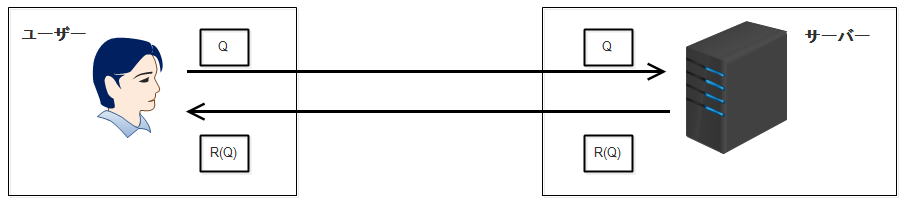
\includegraphics[width=\columnwidth]{photo1.png}
    \end{column}
\end{columns}
	\begin{block}{}
	\begin{itemize}
    	\item Q:検索質問
		\item R(Q):質問Qの検索結果
	\end{itemize}
	\end{block}
\end{frame}

\begin{frame}{Location vs Keyword}
	\begin{block}{}
		\begin{itemize}
		\item Location
			\begin{itemize}
			\item 地図
			\item 乗換案内
			\item 近くのラストラン
			\end{itemize}
		\end{itemize}
        \begin{itemize}
        \item Keyword
            \begin{itemize}
            \item ウェブ検索
            \item データベース検索
            \item クラウドストア検索
            \end{itemize}
        \end{itemize}
	\end{block}
\end{frame}

\begin{frame}{AOL 事件}
	\begin{exampleblock}{AOL質問ログ}
	\fontsize{7pt}{7.2}\selectfont
	\begin{tabular}{ccccc}
	\noalign{\hrule height 1pt}
	AnonID & Query & QueryTime & ItemRank & ClickURL \\
	\hline
	4417749 & care packages & 2006-03-02 09:19:32 & 10 & http://booksforsoldiers.com \\
 	4417749 & care packages & 2006-03-02 09:19:32 & 9 & http://www.brandonblog.com \\
	4417749 & movies for dogs & 2006-03-02 09:24:14 & & \\		
	4417749 & blue book & 2006-03-03 11:48:52 & 1 & http://www.kbb.com \\
	4417749 & best dog for older owner & 2006-03-06 11:48:24 & 1 & http://www.canismajor.com \\
	4417749 & best dog for older owner & 2006-03-06 11:48:24 & 5 & http://dogs.about.com \\
	\noalign{\hrule height 1pt}
	\end{tabular}
	\end{exampleblock}
	\begin{block}{}
	\begin{itemize}
		\item 2006年8月4日、AOL(American OnLine)が650,000人以上のユーザーの匿名化された検索質問ログを研究目的でリリースした。\pause
		\item 2006年8月9日、ID 4417749の名前、年齢、住所などが特定された。\cite{AOL}
	\end{itemize}
	\end{block}
\end{frame}

\begin{frame}{Location vs Keyword}
	\begin{columns}[c]
		\begin{column}{0.3\textwidth} % 横幅の30%
			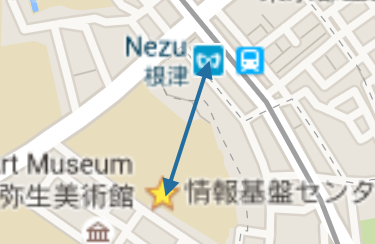
\includegraphics[width=\columnwidth]{photo8.png}
		\end{column}
		\begin{column}{0.3\textwidth} % 横幅の30%
		\begin{center}
			猫 ? 犬
		\end{center}
		\end{column}
	\end{columns}
    \begin{block}{}
    \begin{itemize}
		\item 位置間の距離は簡単に計算できるが、\\ 単語間の距離は計算しにくい
		\item 単語の次元数が高い
   \end{itemize}
    \end{block}
	\begin{columns}[c]
		\begin{column}{0.3\textwidth} % 横幅の30%
			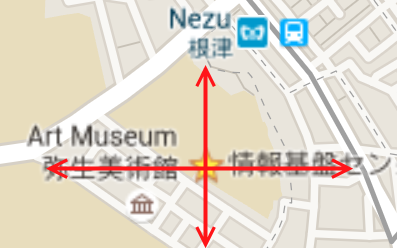
\includegraphics[width=\columnwidth]{photo8-1.png}
		\end{column}
		\begin{column}{0.3\textwidth} % 横幅の30%
		\begin{center}
			猫?
		\end{center}
		\end{column}
	\end{columns}
    \begin{block}{}
    \begin{itemize}
		\item ノイズを加えにくい
    \end{itemize}
    \end{block}
\end{frame}

\section{守り方}
	\begin{frame}{Anonymity}
	\begin{columns}[t]
		\begin{column}{0.8\textwidth} % 横幅の30%
			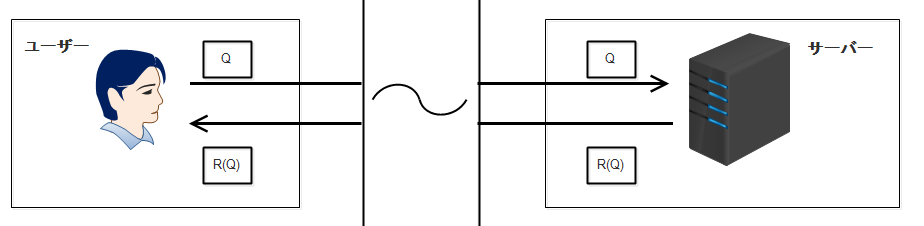
\includegraphics[width=\columnwidth]{photo2.png}
		\end{column}
	\end{columns}

    \begin{block}{}
    \begin{itemize}
		\item 質問者を隠す
    \end{itemize}
    \end{block}
\end{frame}

\begin{frame}{Tursted Third Party}
    \begin{columns}[t]
        \begin{column}{0.8\textwidth} % 横幅の30%
            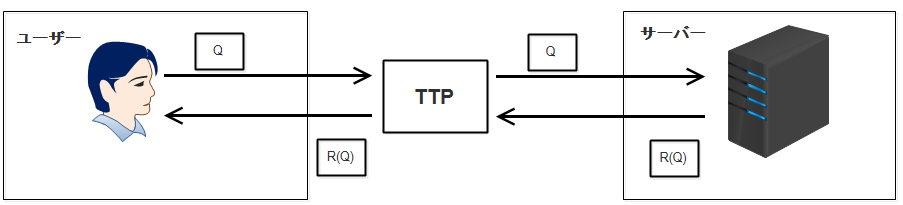
\includegraphics[width=\columnwidth]{photo9.png}
		\end{column}
    \end{columns}
	\begin{block}{} 
		\begin{itemize}
			\item 質問者のIPアドレスなどを隠す
		\end{itemize}
	\end{block}
\end{frame}
\begin{frame}{Tursted Third Party}
    \begin{columns}[t]
        \begin{column}{0.8\textwidth} % 横幅の30%
            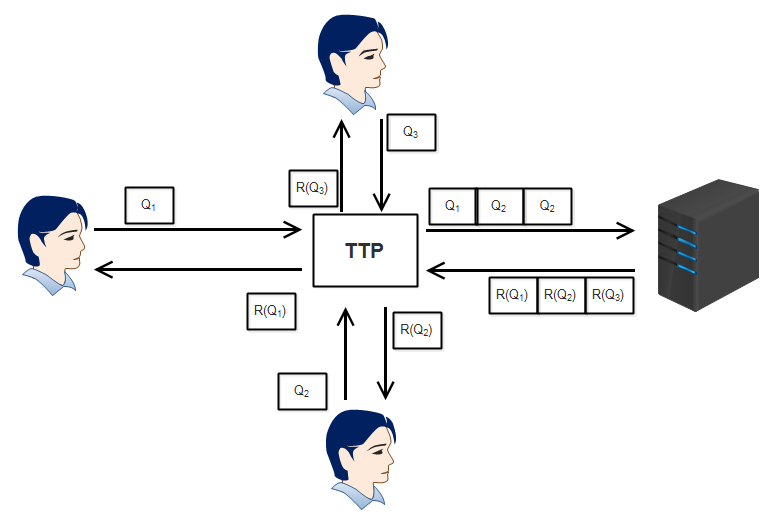
\includegraphics[width=\columnwidth]{photo9-1.png}
		\end{column}
    \end{columns}
	\begin{block}{} 
		\begin{itemize}
			\item 複数の質問者を混ぜて検索する
		\end{itemize}
	\end{block}
\end{frame}

\begin{frame}{Perturbation}
	\begin{exampleblock}{Location}
		\begin{itemize}
			\item Geo-indistinguishability \cite{andres_geo-indistinguishability:_2013}
		\end{itemize}
	\end{exampleblock}
	\begin{exampleblock}{Keyword}
		\begin{itemize}
			\item 質問を一般化して検索する\cite{arampatzis_query_2012}
				\begin{center}
					リンゴ $\Rightarrow$ 赤 果物 
				\end{center}
			\item 事前に標準質問を作って、本当の質問の代わりに使う \cite{murugesan_providing_2009}
		\end{itemize}
	\end{exampleblock}
\end{frame}

\begin{frame}{Obfuscation}
    \begin{columns}[t]
        \begin{column}{1\textwidth} % 横幅の30%
            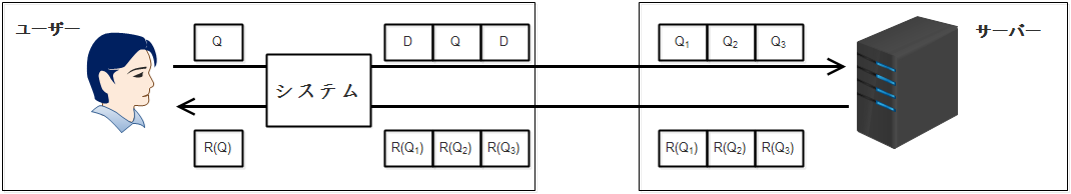
\includegraphics[width=\columnwidth]{photo4.png}
		\end{column}
    \end{columns}
	\begin{block}{} 
		\begin{itemize}
			\item 複数の質問を混ぜて検索する
		\end{itemize}
	\end{block}
\end{frame}

\begin{frame}{Obfuscation-Location}
    \begin{columns}[c]
        \begin{column}{0.4\textwidth} % 横幅の30%
            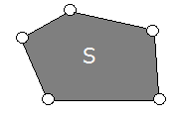
\includegraphics[width=\columnwidth]{photo10.png}
		\end{column}
    \end{columns}
	\begin{Definition}[$(k,s)-privacy$ \cite{lu_pad:_2008}]
		本当の位置と$k-1$個のダミー位置に囲まれた図形の面積が$S$以上ある
	\end{Definition}
\end{frame}

\begin{frame}{Obfuscation-Keyword \cite{balsa_ob-pws:_2012}}
	\begin{block}{問題}
		どうのようなダミー質問がいいダミー質問 \pause
	\end{block}
	\begin{block}{Plausibly Deniable Search \cite{murugesan_providing_2009}}
		\begin{itemize}
			\item 本当の質問との“距離”が遠い
			\item 本当の質問と似たような“確率”で提出される
		\end{itemize}
	\end{block}
\end{frame}

\begin{frame}{Latent Semantic Analysis}
    \begin{columns}[c]
        \begin{column}{1.0\textwidth} % 横幅の30%
            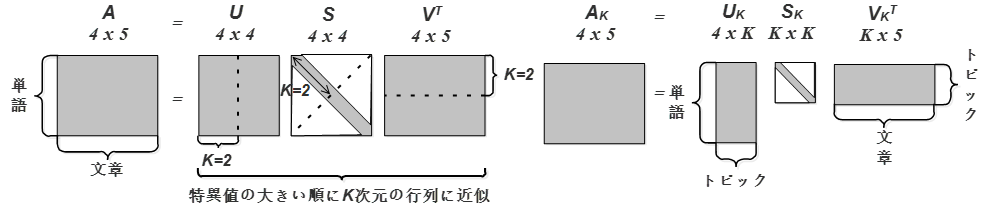
\includegraphics[width=\columnwidth]{photo11.png}
		\end{column}
    \end{columns}
	\begin{block}{潜在的意味インデキシング}
	\fontsize{12pt}{7.2}\selectfont
		単語$\cdot$文書行列$A$を特異値分解$A = USV^T$し、$U$、$S$、$V$	の各列ベクトルを特異値が大きい順に
		$K$個用いて$A$の低ランク近似$A_K=U_KS_KV_{K}^T$を得る。 \\
		このように低ランク分解によって、単語とトピックの関係を分析することができる
	\end{block}
\end{frame}

\begin{frame}{Plausibly}
	\begin{columns}[t]
		\begin{column}{0.8\textwidth} % 横幅の30%
			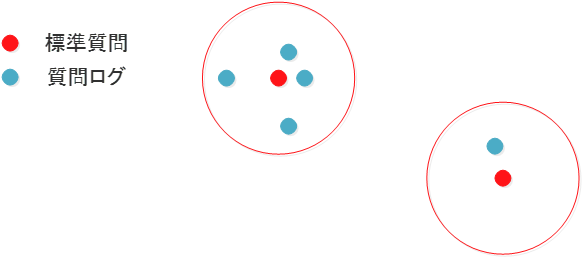
\includegraphics[width=\columnwidth]{photo12.png}
		\end{column}
	\end{columns}
	\begin{block}{} 
		\begin{itemize}
			\item 質問の近傍の中の質問数で“確率”、あるいは尤もらしさを計算する
			\item 質問数が多いほど“確率”が高いとする
		\end{itemize}
	\end{block}
\end{frame}

\begin{frame}{Plausibly Deniable Search}
	\begin{columns}[t]
		\begin{column}{1.0\textwidth} % 横幅の30%
			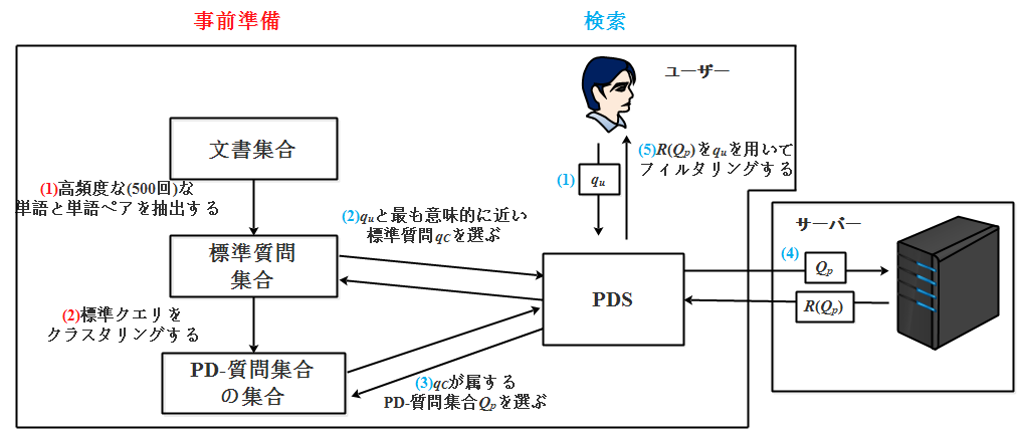
\includegraphics[width=\columnwidth]{photo13.png}
		\end{column}
	\end{columns}
\end{frame}

\begin{frame}{PIR \cite{ostrovsky_survey_2007}}
	\begin{columns}[t]
		\begin{column}{0.8\textwidth} % 横幅の30%
			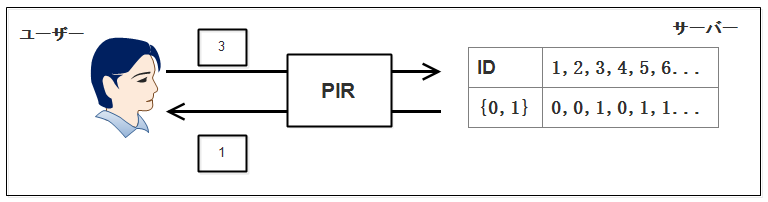
\includegraphics[width=\columnwidth]{photo7.png}
		\end{column}
	\end{columns}
	\begin{block}{} 
		\begin{itemize}
			\item 暗号などの手法を用いて質問の内容を完全に隠す
		\end{itemize}
	\end{block}
\end{frame}

\begin{frame}{凖同型暗号}
	\begin{Definition}[凖同型暗号]
		二つの暗号文 $Enc(m_1), Enc (m_2)$ が与えられた時に、平文や秘密鍵なしで $Enc( m_1 \circ m_2 )$ を計算できる暗号
	\end{Definition}
	\begin{Example}[加算ができる凖同型暗号]
		$Enc(\cdot):$ 暗号化 \, $Dec(\cdot):$復号 \\
		$ Dec(Enc(m_1) \cdot Enc (m_2)) = m_1 + m_2$
	\end{Example}
\end{frame}
\begin{frame}{凖同型暗号}
\fontsize{12pt}{7.2}\selectfont
    \begin{columns}[t]
        \begin{column}{0.5\textwidth}
			\begin{block}{ユーザー} 
			\begin{columns}[t]
				\begin{column}{0.8\textwidth}
				\begin{block}{質問生成}
				\begin{algorithmic}[1]
					\STATE Input:$i^*,n$
					\FOR{$i = 1, \dots, n$}
					\IF{$i == i^*$}
					\STATE {$ q_i = Enc(1)$}
					\ELSE
					\STATE{$ q_i =Enc(0)$}
					\ENDIF
					\ENDFOR
					\RETURN $Q = \{q_1, \dots, q_n\}$
				\end{algorithmic}
				\end{block}
				\begin{block}{復号}
				\begin{algorithmic}[1]
					\STATE input:$R$
					\RETURN $Dec(R)$
				\end{algorithmic}
				\end{block}
				\end{column}
			\end{columns}
			\end{block}
        \end{column}
        \begin{column}{0.5\textwidth}
			\begin{block}{サーバー} 
			\begin{columns}[t]
				\begin{column}{0.8\textwidth}
				\begin{block}{結果計算}
				\begin{algorithmic}[1]
					\STATE Input:$Q,\{x_1, \dots, x_n \}$
					\STATE $R = 0$
					\FOR{$i = 1, \dots, n$}
					\STATE $R = R \cdot q_i^{x_i}$
					\ENDFOR
					\RETURN $R$
				\end{algorithmic}
				\end{block}
				\end{column}
			\end{columns}
			\end{block}
			\begin{block}{Note}
				$m_1 = m_2 \nRightarrow Enc(m_1) = Enc(m_2)$ \\
				$Dec(R) = \sum_{x_i = 1}Dec(q_i) = x_{i^*}$
			\end{block}
        \end{column}
    \end{columns}
\end{frame}

\begin{frame}[t,allowframebreaks]{PIR}
\fontsize{12pt}{7.2}\selectfont
	\begin{block}{}
		\begin{itemize}
			\item 1995 Chor et al. : Multiserver PIR             
			\begin{itemize}
				\item 情報理論から見るとsingle-database PIRができない              
			\end{itemize}
			\item 1997 Kushilevitz and Ostrovsky : computational single-database PIR             
			\begin{itemize}
				\item $quadratic \, residuosity \, computational \, assumption$
				\item  通信量: $O(2^{\sqrt{lognloglogN}})$             
			\end{itemize}
			\item 1999 Cachin et al. : s-PIR            
			\begin{itemize}
				\item $\Phi-hiding \, number-theoretic \, assumption$
				\item  通信量: $O(log^8n)$ 
			\end{itemize}
			\item 2000 Kushilevitz and Ostrovsky : Private Block Retrieval             
			\begin{itemize}
				\item $Naor-Yung \, one-way \, 2-to-1 \, trapdoor \, permutations$
              			\item $Goldreich-Levin hard-core predicates$
				\item  通信量: $n-cn/2k + O(k^2)$ 
			\end{itemize}
		\end{itemize}
	\end{block}
	\begin{block}{}
		\begin{itemize}
			\item 2005 Gentry and Ramzan : Multiserver PIR             
			\begin{itemize}
				\item $\Phi-hiding \, number-theoretic \, assumption$     
				\item  通信量: $O(log^2n)$         
			\end{itemize}
			\item 2007 Aguilar-Melchor and Gaborit : computationally-efficient PIR             
			\begin{itemize}
				\item $lattice-based$
				 \item   a few thousand bit-operations per bit in the database
				 \item 2010 Olumofin and Goldberg:応答時間は普通の方法の千分の一くらい
			\end{itemize}
			\item 2013 Yi et al. : PBR             
			\begin{itemize}
				\item $Fully \, homomorphic \, encryption$
				\item 通信量: $𝑂(\gamma𝑙𝑜𝑔𝑚+\gamma𝑛/𝑚) $
				\item 計算量: $𝑂(𝑚\gamma^2 𝑙𝑜𝑔𝑚+\gamma𝑛/2)𝑏𝑖𝑡 𝑜𝑝𝑒𝑟𝑡𝑎𝑖𝑜𝑛𝑠 $
				\item 計算時間:$2min$
				\item 通信時間: $4.5s(100-Mb/second)$
			\end{itemize}
		\end{itemize}
    	\end{block}
\end{frame}

\begin{frame}{Obfuscation + PIR}
	\begin{block}{Embellishing Text Search Queries to Protect User Privacy \cite{pang_embellishing_2010}}
	    \begin{columns}[t]
			\begin{column}{0.8\textwidth} % 横幅の30%
				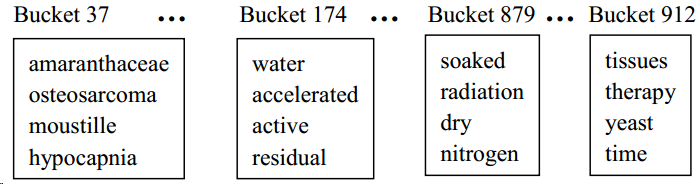
\includegraphics[width=\columnwidth]{photo15.png}
			\end{column}
		\end{columns}
		\begin{itemize}
			\item 本当の質問との“距離”が遠い
			\item 本当の質問と似たような“確率”で提出される
			\item 質問ではなく単語ごとにダミーを加える
		\end{itemize}
	\end{block}
\end{frame}

\begin{frame}{Wordnet}
	\begin{columns}[t]
		\begin{column}{1.0\textwidth} % 横幅の30%
			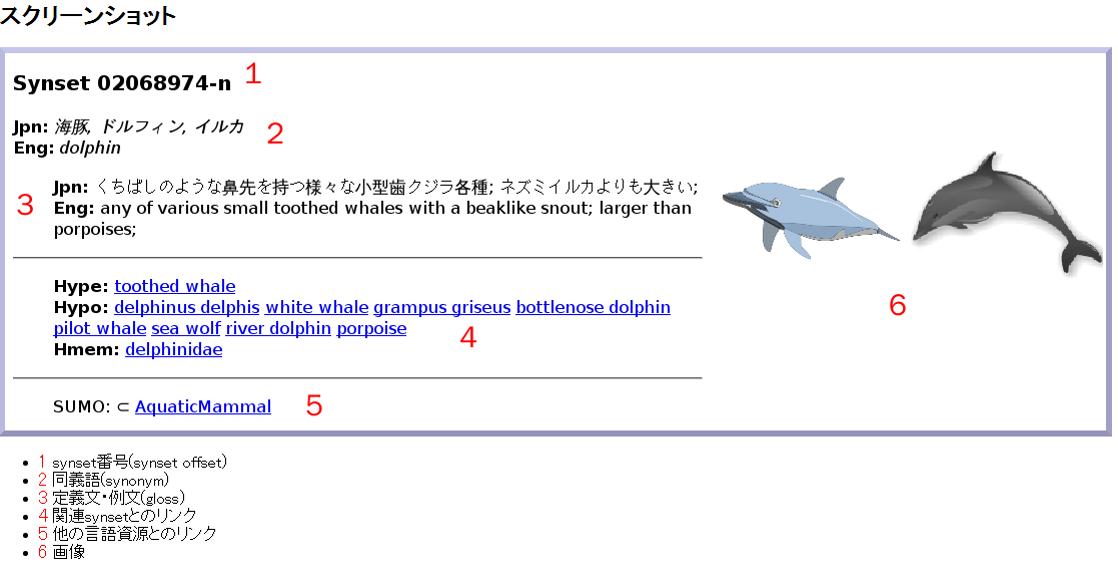
\includegraphics[width=\columnwidth]{photo14.png}
		\end{column}
	\end{columns}
	\begin{block}{}
		\begin{itemize}
			\item “距離”:単語間の最小リンク数
			\item “確率”:単語が属するsynsetのレベル
		\end{itemize}
	\end{block}
\end{frame}
\begin{frame}{Obfuscation + PIR}
\fontsize{12pt}{7.2}\selectfont
	    \begin{columns}[t]
			\begin{column}{0.8\textwidth} % 横幅の30%
				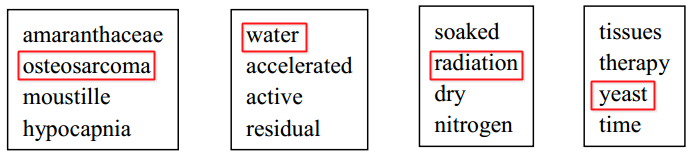
\includegraphics[width=\columnwidth]{photo15-1.png}
			\end{column}
		\end{columns}
    \begin{block}{}
    	$q = \{\langle amaranthaceae,E(0) \rangle , \langle osteosarcoma,E(1) \rangle , \dots \}$ 
    	$t_i:$単語$i\,$ $d_j:$文章$j\,$ $L_i:t_i$の検索結果 $\,p_{ij}:d_j$に対して$t_i$の$score$
    \end{block}
    \begin{block}{Query processing by the search engin}
        \begin{algorithmic}[1]
            \STATE {Input:Embellished query $q$}
            \STATE Let $R = \phi$
            \FORALL {$\langle t_i,E(u_i) \rangle \in q$}
            \FORALL {$\langle d_j,p_{ij} \rangle \in L_i$}
            \IF{$\exists\langle d_j,E(score_j) \rangle \in R$}
            \STATE $E(score_j) = E(score_j) \cdot E(u_i)^{p_{ij}}$
            \ELSE \STATE Insert $\langle d_j,E(u_i)^{p_{ij}} \rangle$ into $R$
            \ENDIF
            \ENDFOR
            \ENDFOR
            \RETURN $R$
        \end{algorithmic}
    \end{block}
\end{frame}

\begin{frame}{Snapshot vs Sequence}
	\begin{block}{Location}
	\end{block}
\end{frame}

\begin{frame}{Snapshot vs Sequence}
	\begin{block}{Keyword}
	    \begin{columns}[t]
			\begin{column}{1.0\textwidth} % 横幅の30%
				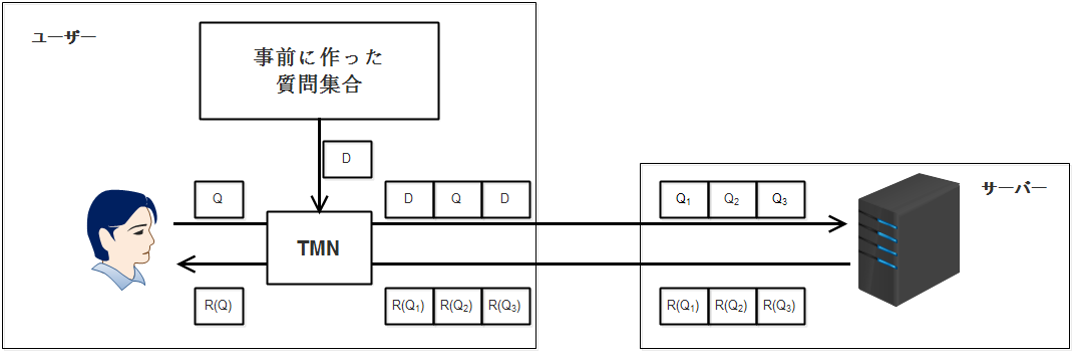
\includegraphics[width=\columnwidth]{photo5.png}
			\end{column}
		\end{columns}
		\begin{block}{TrackMeNot \cite{howe_trackmenot:_2009}}
			一つ一つの質問ではなく、ユーザーの質問ログにノイズを加える
		\end{block}
	\end{block}
\end{frame}

\begin{frame}{Others}
	\begin{exampleblock}{クラウドストア検索}
		\begin{itemize}
			\item CryptDB \cite{popa_cryptdb:_2011}
			\begin{itemize}
				\item ユーザーが自分が暗号化した、クラウド上のデータを暗号化したままで検索する方法
			\end{itemize}
		\end{itemize}
	\end{exampleblock}
   \begin{exampleblock}{データベースの情報を守る}
		\begin{itemize}
			\item Simulatable Auditing \cite{kenthapadi_simulatable_2005}
			\begin{itemize}
				\item ユーザーの差分質問からデータベース上の情報を守る
			\end{itemize}
		\end{itemize}
    \end{exampleblock}

\end{frame}
\section{攻撃方}
\begin{frame}
\end{frame}
\begin{frame}
\end{frame}
\begin{frame}
\end{frame}

\section{参考文献}
\begin{frame}[t,allowframebreaks]{Bibliography}
\fontsize{8pt}{7.2}\selectfont
\bibliographystyle{alpha}
\bibliography{zotero}
\end{frame}

\end{document}
